Here we analyze the behavior of the explicit Linear Steklov method (\SM) for scalar and vector SDEs. 
The tests confirm the convergence order 1/2 for stochastic differential systems with locally Lipschitz drift 
and suggest that the \SM scheme reproduces almost surely stability (a.s.). We validate the efficiency of the new 
method  by comparing with other actual methods like the Euler-Maruyama, Backward-Euler-Maruyama (BEM) \cite{Mao2013} 
and Tamed-Euler-Maruyama (TEM) \cite{Hutzenthaler2012a}. All simulations are implemented in Python 2.7 and we use the 
Mersenne random number generator with fixed seed 100.
	
\begin{example}

		Here we illustrate the stability \Cref{thm:AlmosSurleyStability} through an numerical example presented in 
	\cite[sec 7, pg. 420]{Appleby2010}. Here, \citeauthor{Appleby2010}, proved that the EM method does not satisfies 
	the almost sure stability of the test SDE
	\begin{equation}
	dy(t)= -\beta y(t)|y(t)|^p dt +\sigma(t)|y(t)|^ {\rho} dW(t).
	\end{equation}
	So, the EM approximation explodes to infinity on finite time when $p+1>2\rho$. But, with the same parameters
	%it is known that 
	$
	\lim_{t \to \infty} y(t)=0 \quad \as
	$, see \cite{Appleby2008, Appleby2010} for more details.
	In particular for  the following SDE 
	\begin{equation}\label{eqn:ApplebyEY1}
		dy(t) = -y^3 dt 
		+ \frac{1}{\left[\log(t+1)\right]^{1.1}} dW_t, \qquad t>0,
	\end{equation}
	and deduce conditions for the step-size $h$ and initial condition $y(t_0)=y_0$ in order to claim with high 
	probability
	when the EM scheme for SDE \eqref{eqn:ApplebyEY1} is as-stable or diverge \cite[Cor 7.1 pg. 421]{Appleby2010}. 
	More specifically, given $h<\num{0.0384}$ and  the EM for SDE \eqref{eqn:ApplebyEY1}
	\begin{equation}\label{eqn:EMRecurrenceApplbyEY1}
		X_{k+1} = X_k -h X_k^3 
		+\frac{1}{[\log(n+1)]^{1.1}} \Delta W_k, \qquad X_0=y(t_0).
	\end{equation}
	\begin{enumerate}[(i)]
		\item
		If $
		\displaystyle
		X_0\in \left(
		-\sqrt\frac{2}{h} + 7 \sqrt h,
		\sqrt\frac{2}{h} - 7 \sqrt h
		\right),
		$
		then
		$
		\displaystyle
		\Prob{
			\lim_{k\to\infty}
			X_k = 0
		}>0.95
		$\quad.
		\item  
		If 
		$
		\displaystyle
		X_0\in \left(
		-\infty,
		-\sqrt\frac{2}{h} - 7 \sqrt h
		\right)
		\bigcup
		\left(
		\sqrt\frac{2}{h} + 7 \sqrt h,
		\infty
		\right)
		$,
		then 
		$$
		\displaystyle
		\Prob{
			\limsup_{n\to\infty}
			X_k = \infty
			\text{ or }
			\liminf_{n\to\infty}
			X_k = -\infty
		}>0.95 \quad.
		$$
		
	\end{enumerate}
	Thus we perform a simulation with step size $h=\num{0.2}$  using 
	the EM, Tamed Euler-Maruyama (TEM) and the \SM schemes with unstable EM initial conditions. 
	\Cref{fig:pathsAppleby} shows how the EM scheme produces spurious solutions. Meanwhile, the TEM ans \SM 
	approximations
	reproduce the asymptotic behavior, also we observe a better initial precision of the \SM approximation. 
	\begin{figure}[h]
		\begin{center}
			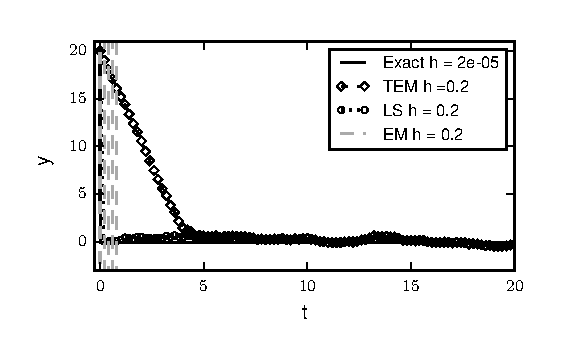
\includegraphics{papers/paperB/figures/ApplebyEx}
		\end{center}
		\caption{Likening between the EM, TEM and \SM approximations with unstable EM conditions. Here "exact" means
			a BEM solution with step size $h=\num{2e-5}$.}
		\label{fig:pathsAppleby}
	\end{figure}
\end{example}

\begin{example} We examine the \SM method using a SDE with super-linear grow diffusion. We 
	consider the SDE reported by \citeauthor*{Tretyakov2013} in \cite[Eq. (5.6)]{Tretyakov2013}
	\begin{equation}\label{eqn:SDETretyakov}
		dy(t) =
		\left(
			1-y^5(t) +y^3(t)  
		\right) dt
		+
		y^2(t) dW(t), \qquad y_0=0.
	\end{equation}
	\citeauthor{Tretyakov2013} show via simulation of \eqref{eqn:SDETretyakov} that the increment-tamed scheme
	\cite[Eq(1.5)]{Hutzenthaler2015}
	\begin{equation}\label{eqn:Increment-Tamed}
		X_{k+1} = X_k + 
		\frac{
			f(X_k) h + 
			g(X_k)\Delta W_k 
		}{
		\max\left(
		1, h
		\left|
		h f(X_k) +
		g(X_k)\Delta W_k
		\right|
	\right)}
	\end{equation}
	produces spurious oscillations. \citeauthor{Hutzenthaler2015} prove the convergence of this scheme under
	linear growth condition over diffusion. So, this suggests us that only certain kind of 
	explicit schemes with convergence under globally Lipschitz and linear growth diffusion conditions	
	%globally Lipschitz diffusion and linear growth 
	can extended their convergence to a locally Lipschitz diffusion and other kind of growth bound.
	Using $a(x):= -x^4 +x^2$, $b: = 1$ and $E=\{-1,0,1\}$, we construct the \SM method
	\begin{equation}\label{eqn:TreyakovLSMethod}
		Y_{k+1} = \exp(ha(Y_k))Y_k + 
		\frac{\exp(ha(Y_k)) - 1}{a(Y_k)} \1{E^c}
		+h\1{E}
		+Y_k^2\Delta W_k. 		
	\end{equation}
	\Cref{fig:Tretyakov} shows the numerical solution of SDE \eqref{eqn:SDETretyakov} with the Increment-Tamed (I-TEM) 
	\eqref{eqn:Increment-Tamed}, \SM method \eqref{eqn:TreyakovLSMethod}, and the Tamed (TEM) scheme. 
	We consider the implicit Midpoint scheme \cite[Eq.(5.3)]{Tretyakov2013} with $h=\num{e-4}$ 	as reference.
	\begin{figure}[h!]
		\centering
		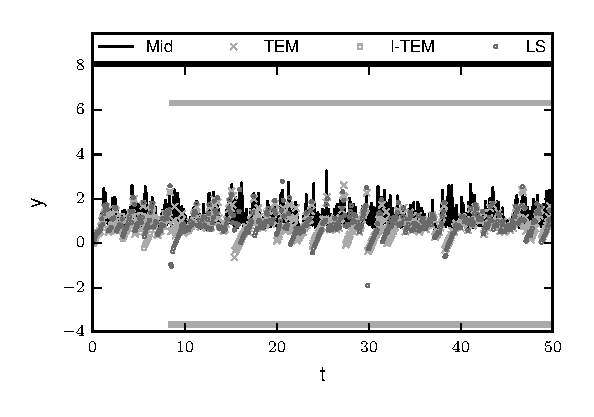
\includegraphics{./papers/paperB/figures/Tretyakov}
		\caption{
			Numerical solution of SDE \eqref{eqn:SDETretyakov} using the I-TEM 
			\eqref{eqn:Increment-Tamed}, \SM method \eqref{eqn:TreyakovLSMethod}  and TEM
			with $h=\num{0.1}$. The reference solution is a Midpoint rule approximation with $h=\num{e-4}$.
		}
		\label{fig:Tretyakov}
	\end{figure}
\end{example}

\begin{example}
	Now we compare the order of convergence and the run time of the \SM method with the TEM scheme as in 
	\cite{Hutzenthaler2012a}. That is, we consider a  Langevin equation under  the $d$-dimensional potential 
	$U(x)= \frac{1}{4}|x|^4 - \frac{1}{2}|x|^2$, and $d$-dimensional Brownian additive noise. The corresponding
	SDE reads
	\begin{equation}\label{eqn:SDELangevinHutz}
	dy(t) = 
		\left(
			y(t) - |y(t)| \cdot y(t)
		\right)dt
		+ dW(t), \qquad y(0)=0.
	\end{equation}
	This model describes the motion of a Brownian particle of unit mass immersed on the potential $U(x)$. 
	Taking $a_j(x):=1-|x|$ and $b_j=0$, $j\in \{1,\dots, d\}$ we obtain the \SM method
	\begin{equation}\label{eqn:LangevinLSMethod}
		Y_{k+1} = \diag
		\left[		
			e^{h a_1(Y_k)}, \dots, e^{ha_d(Y_k)}) 
		\right] 
		Y_k+
		\Delta W_k.
	\end{equation}
	\Cref{tbl:OrdersLS} shows the root means square errors at a final time $T=1$, which is approximated by
	\begin{equation}
		\sqrt{\EX{|Y_N - y(T)|^2}} \approx 
		\frac{1}{M}
		\left(
		\sum_{i=1}^M
		|y_i(T) - Y_{N,i}|^2	
		\right)^{1/2},
	\end{equation}
	over a sample of $M$ =\num{10000} trajectories of the TEM, \SM  and BEM solutions to SDE 
	\eqref{eqn:SDELangevinHutz} with dimension $d=10$.  We consider the TEM solution with step $h=2^{-19}$ as reference 
	solution. 
	In this experiment we confirm that the \SM method converges with standard order 1/2  and is almost equal accurate 
	as the TEM approximation.

		In some applicationa as in Browninan Dynamics Simulations \cite{Cruz2012}, the dimension of a SDE
	increases considerable the complexity and computational cost --- this excludes the use of implicit methods.
	In \Cref{fig:TimeVsDimension}, we observe that the runtime of the BEM method grows quadratically depending
	on the dimension, meanwhile the LS and TEM methods grow linearly. 
	\begin{table}[t]
		\centering
		\begin{tabular}{lllllll}
			&        TEM &        	& LS		&           & BEM		 &         \\
			\toprule
			h		& ms-error	 & ECO 		& ms-error	    & ECO		& ms-error	 &	ECO	  \\
			\midrule
			$2^{-2}$	& \num{1.70388}    & ---		&\num{1.55394}		& ---		& \num{1.38157}	& 
			--- \\
			$2^{-3}$	& \num{1.16977}    & \num{0.54}     &\num{1.10775}    & \num{0.48} & \num{1.05309}	& 
			\num{0.39} \\ 
			$2^{-7}$	&\num{0.27895}     & \num{0.48} & \num{0.27795}   & \num{0.48} & \num{0.276895}& 
			\num{0.48} \\
			$2^{-11}$	& \num{0.07010}  & \num{0.50} & \num{0.07009}  & \num{0.50} & \num{0.07007} & 
			\num{0.50} \\
			$2^{-15}$	& \num{0.01739}  & \num{0.51} & \num{0.01739}  & \num{0.51} & \num{0.01739}& 
			\num{0.51} \\
			\bottomrule
		\end{tabular}
		\caption{
			Mean square errors and the experimental convergence order (ECO) for the SDE \eqref{eqn:SDELangevinHutz} 
			with a TEM with $h = 2^{-19}$ as reference solution.
		}\label{tbl:OrdersLS}
	\end{table}
	\begin{figure}[t]
		\centering
			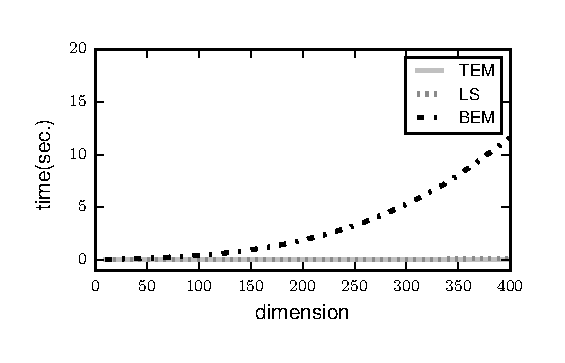
\includegraphics{./papers/paperB/figures/TimeVsDimension}
		\caption{
			Runtime calculation of $Y_N$ with $h=2^{-17}$, using the BEM,  \SM and TEM methods for 
			SDE \eqref{eqn:SDELangevinHutz}.
		}
		\label{fig:TimeVsDimension}
	\end{figure}
\end{example}

\begin{example}
	Let us recall the following  stochastic model for internal 
	HIV dynamics given by  \citeauthor{Dalal2008} in \cite{Dalal2008}:
	\begin{align}\label{eqn:StochasticHIVDynamics}
		dy_1(t) &=
		\left(
			\lambda -\delta y_1(t) - (1 - \gamma) \beta y_1(t) y_3(t)
		\right)dt
		-\sigma_1 y_1(t) dW^{(1)}_t, 
		\notag \\
		dy_2(t) &= 	
		\left(
			(1- \gamma) \beta y_1(t) y_3(t) - \alpha y_2(t) 
		\right)dt
		-\sigma_1 y_2(t) dW^{(1)}_t, 
		\\
		dy_3(t) & = 
		\left(
			(1 - \eta) N_0 \alpha y_2(t) 
				-\mu y_3(t)
			-(1 - \gamma ) \beta y_1(t) y_3(t) 
		\right)dt
		- \sigma_2 y_3(t) dW^{(2)}_t.
		\notag
	\end{align}	
	\begin{figure}[h!]
		\centering
		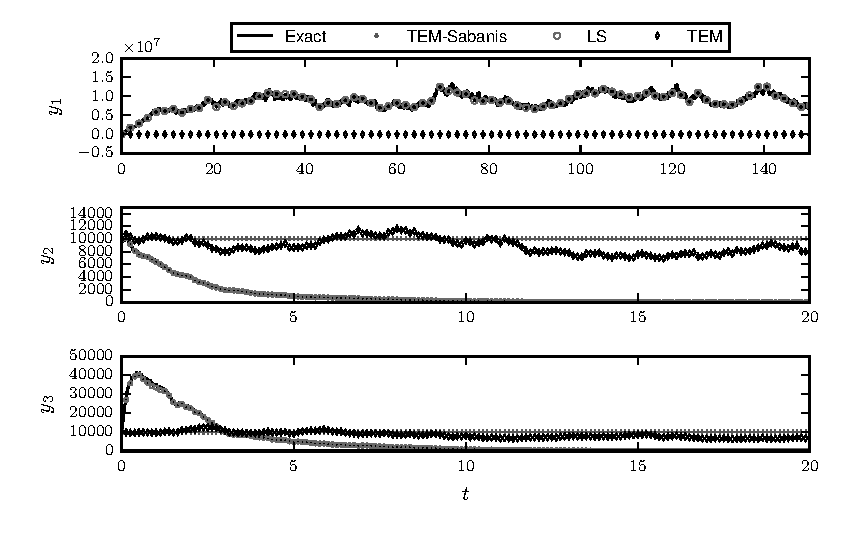
\includegraphics{./papers/paperB/figures/InternalHIVDynamics}
		\caption{
			Likening between EM, \SM, TEM approximations for SDE \eqref{eqn:StochasticHIVDynamics} with
			$\gamma = \num{0.5}$,
			$\eta = \num{0.5}$,
			$\lambda = \num{e6}$, 
			$\delta = \num{0.1}$,
			$\beta = \num{e-8}$,
			$\alpha = \num{0.5}$,
			$N_0= \num{100}$,
			$\mu = \num{5}$,
			$\sigma_1 = \num{0.1}$,
			$\sigma_2 = \num{0.1} $,
			$y_0 = (
			\num{10000},%{\per\cubic\deci\meter}, 
			\num{10000},%{\per\cubic\deci\meter}, 
			\num{10000}.%{\per\cubic\deci\meter}
			)^T$,
			$h=\num{0.125}$.
			Here the reference solution means a BEM simulation
			with the same parameters but with a step-size $h=\num{e-5}$.
		}
		\label{fig:InternalHIVDynamics5e-1}
	\end{figure} 
	Under certain conditions \citeauthor{Dalal2008} prove 
	that  system \eqref{eqn:StochasticHIVDynamics} has a unique 
	almost surely exponential stability solution, that is,  $y=(y_1,y_2,y_3)$  tends 
	exponentially to an equilibrium $(\bar{y}_1,0,0)$ with probability 1. 
	Now, we want to verify if  the EM, TEM, TEM-Sabanis \cite{Sabanis2015} and LS approximations can reproduce this 
	property of the solution. Taking 
	\begin{align*}
		E_1&:=\left\{
			(x,y,z)^T \in \R^3:
			z=0 
			\text{ or }
			z=0
			\frac{-\delta}{\beta(1-\gamma)}
		\right\}, \quad
		E_2:=	\emptyset,   \\
		E_3&:=\left\{
			(x,y,z)^T \in \R^3: 
			x=0
			\text{ or }
			x=
			\frac{-\mu}{\beta(1-\gamma)}
		\right\}
	\end{align*}
	 
	The LS method for \eqref{eqn:StochasticHIVDynamics} is given by
	
	\begin{align}
		a_{1}(Y_k)) &:= 
		-\left(
		\delta + (1 - \gamma) \beta Y_k^{(3)}
		\right),		
		& b_1(Y_k^{(-1)}) &:= \lambda, 
		& 
		\notag
		\\
		a_{2}(Y_k) &:= -\alpha,
		&b_2(Y_k^{(-2)}) & :=
		(1-\gamma) \beta Y_{k}^{(1)} Y_{k}^{(3)},
		\notag
		\\
		a_{3}(Y_k) &= 
		-
		\left(
		\mu + (1- \gamma) \beta Y_{k}^{(1)}
		\right),
		\qquad
		%
		&b_{3}(Y_k^{(-3)}) &:= 
		\left(
		1 - \eta 
		\right)
		N_0 \alpha Y_{k}^{(2)},
		\notag			
	\end{align}
	the \SM method for the stochastic model \eqref{eqn:StochasticHIVDynamics} reads,
	\begin{align}
		Y_{k+1} &= A^{(1)}(h,Y_k) \,Y_k + A^{(2)}(h,Y_k)b(Y_k)+ g(Y_k)\, \Delta W_k,
		\qquad \Delta W_k = \left(W_k^{(1)}, W_k^{(2)}\right)^T, 
		\notag\\ 
		A^{(1)}(h,Y_k)&:=
		\begin{pmatrix}
			e^{ha_1(Y_k)}	&	0	&0 \\
			0	&e^{ha_2(Y_k))}	&0\\
			0	&0				&e^{ha_3(Y_k))}
		\end{pmatrix},
		%	
		\notag
		\\
		%	
		A^{(2)}&:=
		\begin{pmatrix}
			h \Phi_1(Y_k)\1{E_1^c}	&0	&0\\
			0 & 
			\left(\displaystyle
			\frac{e^{-h\alpha} - 1}{\alpha}
			\right) & 0\\
			0 & 0 & h \Phi_3(Y_k)\1{E_3^c} 
		\end{pmatrix}
		%\notag \\
		+h
		\begin{pmatrix}
			\1{E_1}	&0 			&0\\
			0		&0			&0\\
			0		&0			&\1{E_3}\\
		\end{pmatrix},
	\notag
	\\
	b(Y_k) &:=
	\begin{pmatrix}
		b_1(Y_k^{(-1)})\\
		b_2(Y_k^{(-2)})\\
		b_3(Y_k^{(-3)})
	\end{pmatrix},
	\qquad
	g(Y_k):=
	\begin{pmatrix}
		-\sigma_1 Y_k^{(1)}	&0\\
		-\sigma_1 Y_k^{(2)}	&0\\
		0	&-\sigma_2 Y_k^{(3)}
	\end{pmatrix}.
\end{align}
%
	\Cref{fig:InternalHIVDynamics5e-1} shows the  \SM, TEM and TEM-Sabanis approximations
	with the parameters reported in \cite{Dalal2008}.  The EM approximation
	blows up  so it is not drawn. We observe how the TEM approximation (components $y_2$ and $y_3$) oscillates about 
	the initial condition and the 
	TEM-Sabanis approximation (components $y_2$ and $y_3$) is constant and equal to the initial value, while the \SM 
	method reproduces the asymptotic behaviour of the solution. It is important to remark that the Tamed family methods	
	improve convergence of the Euler method by taming the drift increment term with 
	the factor	$1/(1 + h |f(Y_k)|)$, bounding the norm of  $h f(Y_k)/(1 + h |f(Y_k)|)$ by 1. This norm   
	controls the drift contribution of the Tamed methods  at each step. Such modification 
	is recommended for SDEs with drift contributions and initial conditions with similar scales. We observe
	that for models where such terms have different scales the TEM over damps the drift contribution. 
\end{example}

